\begin{tikzpicture}
\node[minimum width=15cm,minimum height=9cm] (current page) {};
\begin{scope}[overlay]

\begin{visibleenv}<2>
    \node[anchor=north,draw=red,ultra thick,fill=white] (token) at ([yshift=-1cm]current page.north) {
    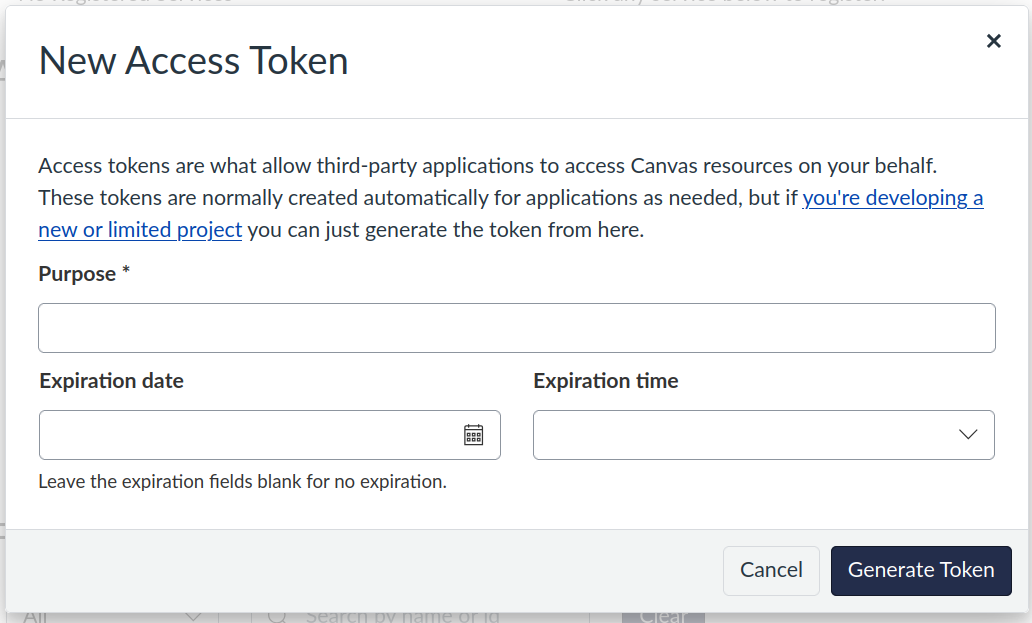
\includegraphics[height=0.6\mypaperheight,alt={Canvas's dialog labeled `New Access Token'. Says `Access tokens are what allow third-party applications to access Canvas resources on your benhalf. These tokens are normally created autommatically for applications as needed, ut if you're developing a new or limited project you can just generate the token from here.' and has a prompt for information and a `Generate Token' button.}]{../http/http-bearer-make-canvas}
};
\end{visibleenv}
\end{scope}
\end{tikzpicture}
